\section{Preliminaries} \label{sec:prelim} 

In this section we first describe the state-of-the-art approach,
\LeeWave{}, for answering distributed $k$NN queries for a
\emph{single} time series. Then we formally define our distributed
\emph{multiple} time series query problem and discuss why the prior
approach is inadequate for dealing with the proposed problem.


\vspace{-0.1in}
\subsection{Distributed $k$NN for Single Time Series}\label{subsec:single}

The conventional $k$NN (or $k$FN) search for a single reference time
series aims at finding $k$ time series of the smallest (largest)
distance to a given reference time series. In this paper, we will
focus on the Euclidean distance: Given two time series
$\Sref$ and $S_x$ of length $T$, $Dst(\Sref,S_x)$ is defined to be
the squared sum of the Euclidean distance between them.  Namely,
{\small
\begin{equation}\label{eq:squareED} 
Dst(\Sref,S_x)=\sum_{i=1}^{T}{(\Sref[i]-S_x[i])^2},
\end{equation}
}
\noindent\hspace{-0.1in}
where $\Sref[i]$ and $S_x[i]$ are the values of $\Sref$ and $S_x$,
respectively, at timestamp $i$.

To deal with time series matching problems, Wavelet transformation,
especially the Haar Wavelet~\cite{HAA05ZUR}, has been applied in a
variety of studies~\cite{Yeh:2008:LLD,Kashyap:2011:SKS,ZHU03EFF}. In
% as~\cite{BUL03SWA,Kashyap:2011:SKS,TEN04RES,Yeh:2008:LLD,ZHU03EFF}. In
Haar wavelet decomposition, each time series is decomposed into
multiple resolutions and can be represented using an error tree
structure~\cite{MAT98WAV}, as shown in
Fig.~\ref{fig:error-tree}(a). Note that only the non-leaf node
coefficients are retained. The notation $n_{(l,p)}^{(u)}$ shown
in Fig.~\ref{fig:error-tree}(b) is used to represent the coefficient
at level $l$ having offset $p$ of time series $S_u$.

\begin{figure}[t!]
%\vspace{1.75in}
%%\special{psfile=error-tree.eps hscale=32 vscale=32 hoffset=-15 voffset=-150}
%\special{psfile=error-tree.eps hscale=40 vscale=40 hoffset=-20 voffset=-200}
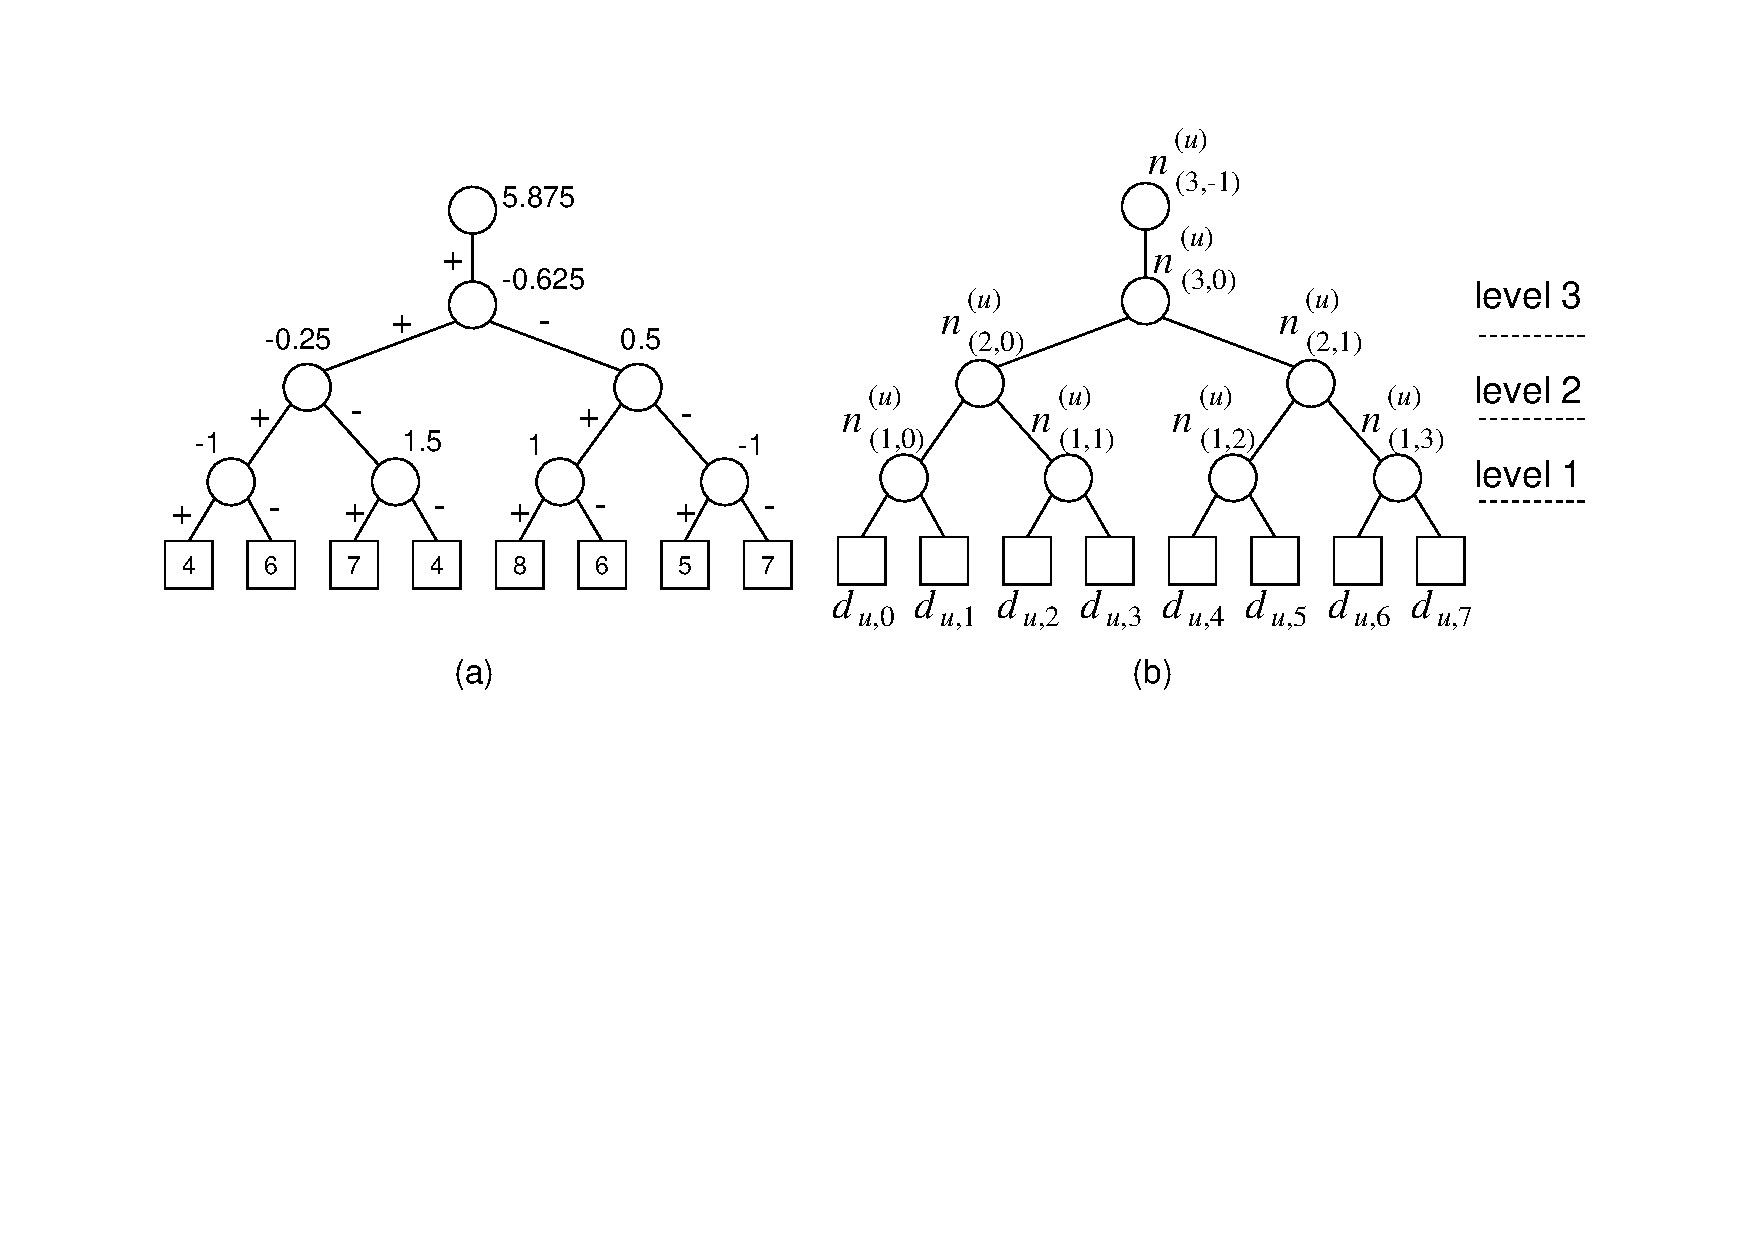
\includegraphics[width=\linewidth]{error-tree.pdf}
\vspace{-0.2in}
\caption{(a) Error tree for a time series \{4,6,7,4,8,6,5,7\}
(b) Error tree notation}
\label{fig:error-tree}
\end{figure}

Given wavelet coefficients of two time series, $Dst(\Sref,S_x)$
can be calculated directly from the coefficients themselves, in a top-down
level-wise manner as suggested in \LeeWave{}~\cite{Yeh:2008:LLD}: 
{\small
\begin{eqnarray}
\lefteqn{Dst(\Sref,S_{x}) = \sum_{l=1}^{L}Dst^{l}(\Sref,S_{x})} \notag \\
& = & accDst^{\ell }(\Sref,S_{x})+\sum_{l=1}^{\ell-1}Dst^{l}(\Sref,S_{x}),
 \label{eq:truedistance} 
\end{eqnarray}
\noindent
where
\begin{equation*}
Dst^{l}(\Sref,S_x)= 2^{l} \times \sum_{p}[n_{(l,p)}^{(\supref)}-n_{(l,p)}^{(x)}]^{2},
\end{equation*}\vspace{-0.1in}
\begin{equation*}
accDst^{\ell}(\Sref,S_x)=\sum_{l =\ell}^{L}Dst^{l }(\Sref,S_x),
\end{equation*}}
\noindent\hspace{-0.1in}
$\ell$ represents the current level, and $L$ is the height of the error tree.

In \LeeWave{}, instead of simultaneously distributing all the relevant
coefficients of the reference series $\Sref$ to all the local machines,
the server only sends the coefficients one level at a time, starting
from the top (the coarsest) level.\footnote{\label{fnt:T}Note
that when the length of a time series is not a power of 2, the
corresponding wavelet coefficients can be represented with multiple
error trees of different heights because any integer value can always
be represented as the summation of distinct powers of two. In such
cases, we still send coefficients from different
sub-trees in a level-wise manner.} Each local machine responds with the
level distance $Dst^{l}(\Sref,S_x)$ for its time series $S_x$ (each machine has
just one time series). Using
such information, the server can determine the similarity range (i.e.,
upper/lower bounds) of each local time series to the reference series:
{\small
\begin{eqnarray}\label{eq:upper-bound}
\lefteqn{accDst^{\ell }(\Sref,S_{x}) \leq Dst(\Sref,S_{x}) \leq} \notag\\
&& accDst^{\ell }(\Sref,S_{x})+\sum_{l=1}^{\ell-1}
  \sum_{p}([n_{(l,p)}^{(\supref)}]^{2}+[n_{(l,p)}^{(x)}]^{2}) \times 2^{l} \notag \\
&& +\ 2 \times \sqrt{\sum_{l=1}^{\ell-1}\sum_{p}[n_{(l,p)}^{(\supref)}\times
  2^{l}]^{2}\times \sum_{l=1}^{\ell-1}\sum_{p}[n_{(l,p)}^{(x)}]^{2}}. 
\end{eqnarray}}

\noindent
Based on these bounds, the server progressively (level-wise) informs
each local machine as to whether its time series is still a candidate for
$k$NN, and if not, the machine drops out of the computation.

Note that the server can compute the lower and upper bounds in
Eq.~(\ref{eq:upper-bound}) from its $n_{(l,p)}^{(\supref)}$ terms and three
summation terms provided by a local machine.  This saves considerable
bandwidth compared to the local machine sending its complete time series.
Also, our earlier work~\cite{Yeh:2008:LLD} proved that the derived upper
bound is non-increasing and the lower bound is non-decreasing when
moving from one level to the next. These increasingly tightened
similarity ranges enable effective pruning of candidates without any
false dismissals.

\vspace{-0.1in}
\subsection{Defining Distributed $k$NN/$k$FN Search for Multiple Time Series}

Before discussing the limitations of the above framework, we first
formulate the distributed $k$NN and $k$FN search problem for multiple
time series.

Let $Q=\{S_{q1},\ldots,S_{qn}\}$ be a set of
$n$ reference time series of length $T$. To match a candidate time
series to the given set of multiple time series, we propose the
following three linkage distances.
\begin{definition} \label{def:3distances}
The \emph{single-link}, \emph{average-link}, and \emph{complete-link}
distances of a time series $S_x$ to a reference set
$Q=\{S_{q1},\ldots,S_{qn}\}$ are defined as:
{\small
\begin{eqnarray*}
d_{sin}(Q, S_x) & = & \min_{1\leq i \leq n}Dst(S_{qi},S_x), \\
d_{avg}(Q, S_x) & = & \sum_{i=1}^{n} Dst(S_{qi},S_x)/n, \text{ and}\\
d_{com}(Q, S_x) & = & \max_{1\leq i \leq n}Dst(S_{qi},S_x). 
\hspace{0.5in}
\end{eqnarray*}}
\end{definition}

These definitions are intended to be analogous to the single-link, average-link, and
complete-link distances used in clustering.  Intuitively, a time
series $S_x$ is considered close to a group of time series $Q$ if either
there exists one time series in $Q$ that is very similar to $S_x$
(i.e., $d_{sin}$), or most of the time series in $Q$ are close
enough to $S_x$ to make their average similar to $S_x$ (i.e., $d_{avg}$), 
or the most dissimilar time series in $Q$ is
still similar to $S_x$ (i.e., $d_{com}$).

With Definition~\ref{def:3distances}, we can now define the distributed $k$NN and
$k$FN search problem for multiple time series queries, referring to Fig.~\ref{fig:system-model}.

\begin{definition}
Given a server $P$ with a reference time series set
$Q=\{S_{q1},\ldots,S_{qn}\}$, each of length $T$, and a set of
distributed local machines $M_1,\ldots,M_m$, each with one or more
time series of length $T$, a \emph{distributed $k$NN ($k$FN) search
for query $Q$} is to find the exact $k$ time series among all the
machines that have the smallest (largest, respectively) linkage
distance, either single-link, average-link, or complete-link as
predefined by the user.  \hfill
\end{definition}

\vspace{-0.1in}
\subsection{Limitations of the Existing Framework}
\label{subsec:limitations}

One immediate question is whether the \LeeWave{} framework from
Section~\ref{subsec:single} can be exploited directly to handle the
multiple time series case.  A simple idea would be to use \LeeWave{}
independently for each of the time series in $Q$, and then try to use
these answers to re-construct the overall $k$NN according to
$d_{sin}$, $d_{avg}$, or $d_{com}$.  We call this framework
\LeeWave-M{}. Unfortunately, considering the 6 cases (3 linkage distance measurements for 
2 kinds of queries), \LeeWave-M{} can guarantee correct
solutions for only 2 of the 6, namely, for $d_{sin}$ in $k$NN and
$d_{com}$ in $k$FN.  To see this, consider the following simple counterexample
for $1$NN search.
\begin{example}
Suppose we have a two length-1 reference time series $S_{q1}$ = \{2\},
$S_{q2}$ = \{-2\}, and candidate time series $S_1$ = \{0\},
$S_2$=\{3\}, and $S_3$=\{-3\} stored in local machine $M_1$ and
candidate time series $S_4$=\{4\} and $S_5$=\{5\} stored in local
machine $M_2$. For $M_1$, $S_2$ gets returned for $S_{q1}$ and $S_3$
for $S_{q2}$; while for $M_2$, $S_4$ gets returned for both reference
series. Considering both machines, $S_2$ is the $1$NN for $S_{q1}$ and
$S_3$ is the $1$NN for $S_{q2}$.  However, the true $1$NN results
under $d_{avg}(Q, S_x)$ and $d_{com}(Q, S_x)$ are both $S_1$, which
was not even selected to be returned to the server.
\end{example}

Similarly, we can find counterexamples for $k$FN under $d_{sin}$ and $d_{avg}$.

Besides the limitation of being able to solve only 2 out of the 6
cases, directly apply \LeeWave-M{} cannot be considered a
bandwidth-efficient approach because each reference series in $Q$ is
processed independently.

The third limitation of \LeeWave{} lies in its server-oriented
computation strategy.  Most of the bounds are calculated on the server
machine based on sum terms sent by the local machines; for the multiple
time series scenario, this strategy wastes bandwidth.

In this paper, we introduce the \MSWave{} framework to deal with the
above limitations.

%In the following, we will introduce how our \MSWave\/ approach solve these challenges. Essentially, the server disseminates the reference time series set in a level-wise manner similar to that in \LeeWave\/. To guarantee no false dismissal when searching for $k$ nearest neighbors to the reference set with only partial information, we show the new bounding computation for the similarity ranges of the three linkage distances of a time series to the reference set. Furthermore, as the reference time series we deal with in \MSWave\/ is multiple, we shift the role of computing the similarity range for each reference-set/candidate-series pair from the server to the local machines. In this way, we can save another significant bandwidth usage compared to the original \LeeWave\/ scheme. Finally, we will show that the same similarity ranges for $k$NN queires can also be used to find the $k$ furthest neighbors.
   




